\section{Introduction}
In location-privacy applications, a verifier may need to establish that a user satisfies a spatial policy without learning the user's precise coordinates. Zero-knowledge location proofs, for example, can verify membership in a designated region while keeping the location private ~\citep{ZKLP,VehiclePolicy}. Such verification commonly starts from a definite spacetime position. Vehicle sensing, however, cannot always provide an observation of that kind. Positioning error, environmental interference, and clock-synchronization uncertainty may restrict the available evidence to a range of plausible positions and times. A valid source signature authenticates the evidence submitted by that source; it does not establish that the physical estimate is accurate. Compromised sources may also sign deliberately misleading observations. Consequently, even a mathematically correct proof concerning a hidden coordinate does not establish that the chosen coordinate is sufficiently supported by observations. This paper asks how multiple uncertain, and potentially malicious, spacetime observations can support a policy-compliance claim without being disclosed to the verifier.

The problem is particularly relevant to vehicular crowdsensing. Distributed vehicle observations support traffic monitoring, road management, and environmental-sensing tasks ~\citep{Suhag2023,Zheng2025BARM}, for which the admissibility of a report may depend on the event's location and time. Revealing the positioning evidence can expose a vehicle's mobility history. Replacing several interval-valued observations with one representative point, however, can conceal disagreement near a policy boundary. Requiring every source interval to intersect is not necessarily safer: a Byzantine issuer may submit a displaced interval that excludes the true state while leaving a small intersection entirely within the authorized region. A sound compliance rule therefore needs to specify which possible states have sufficient evidential support and how conflicting observations are handled, in addition to protecting those observations.

We consider privacy-preserving compliance certification over signed spacetime uncertainty evidence. Each enrolled issuer signs an axis-aligned integer box for the same reference event. For $n$ issuers, at most $f$ Byzantine sources, and at most $r$ honest observations that fail to cover the true state, let $k = n - f - r$. The robust feasible set $\mathcal{F}_k$ consists of the states covered by at least $k$ signed boxes. Compliance is certified only if this set is nonempty and entirely contained in the authorized policy. A nonempty feasible set lying outside the policy produces an invalid decision; a set crossing the boundary is ambiguous; and a set with no threshold-supported state is inconsistent. A valid decision is reserved for the acceptance condition. These four outcomes avoid treating an arbitrarily chosen point as conclusive and distinguish a conflict in otherwise valid evidence from failure to submit the required evidence.

The support-depth construction builds on classical fault-tolerant interval fusion, including the threshold-intersection principle of Marzullo; our contribution is its exact zero-knowledge certification, circuit construction, and report-bound gateway enforcement.

We combine threshold-based fault-tolerant interval reasoning ~\citep{Marzullo1990,BFTPoLoc,PG,CRSF} with zero-knowledge certification. Rather than revealing the source intervals, the prover establishes that the signatures satisfy the roster and context constraints and that the reported decision follows from the same threshold rule. A report-binding protocol associates this proof with the task, issuer roster, report bytes, threshold, challenge nonce, and expiry. This association prevents a proof for one authorized context from being reused as evidence for another, under the stated cryptographic and gateway assumptions.

In a conventional gateway-side fusion design, submitting each signed uncertainty box to the verifier would reveal sensitive spatiotemporal positioning envelopes and make them available for retention or cross-task linkage. Our setting instead permits the gateway to learn the task context, report and final classification, but not the source boxes or their signed private witness. This asymmetry motivates an exact zero-knowledge certificate rather than merely running the threshold rule on disclosed evidence.

Designed as a modular evidence-certification component for vehicular crowdsensing architectures, our framework focuses on source authentication, contextual binding, and verifiable set-level compliance, while treating participant recruitment, incentive mechanisms, and physical sensor calibration as orthogonal upstream services. We explicitly separate these physical coverage premises from cryptographic guarantees throughout the security analysis.

The contributions are summarized as follows:
\begin{itemize}
\item \textbf{Four-valued certification under explicit fault and coverage budgets.} We use the set of threshold-supported spacetime states as the object of policy verification, distinguish valid, invalid, ambiguous, and inconsistent evidence, and establish conditional soundness when the true state is covered by sufficiently many honest sources.
\item \textbf{Two exact finite-domain proof circuits.} Lower-corner maximum-depth reachability and threshold-subset enumeration establish the same four-valued relation. Both are instantiated with Groth16/BN254, verify EdDSA/MiMC signatures within the circuit, and constrain the private evidence to the public policy, roster, threshold, and report context.
\item \textbf{A task-bound verification gateway.} The gateway reconstructs public inputs from a trusted task configuration, checks roster consistency, verifies the proof, and atomically marks a successfully used challenge as consumed. Protocol tests examine evidence tampering, task/report substitution, expired challenges, and concurrent replay within one gateway instance.
\item \textbf{Comprehensive semantic and cryptographic evaluation.} We evaluate the framework across 64,800 synthetic observations, paired ablations over honest-miscoverage allowances, trajectory replay on 787 measured UrbanNav reference states with simulated multisource evidence, 300 Groth16 proof executions across both circuit backends, resource-limited R1CS compilation sweeps, and a same-runner comparison against an open-source location-proof baseline.
\end{itemize}

Figure~\ref{fig:architecture} depicts the certificate workflow. Issuers authenticate uncertainty regions associated with the same report; the vehicle uses the regions and signatures as a private witness; and the gateway checks the public task context and accepts the report only after verifying a valid classification. The witness is hidden from the verifier, while the report content, public policy, and classification remain visible.

\begin{figure}[htbp]\centering
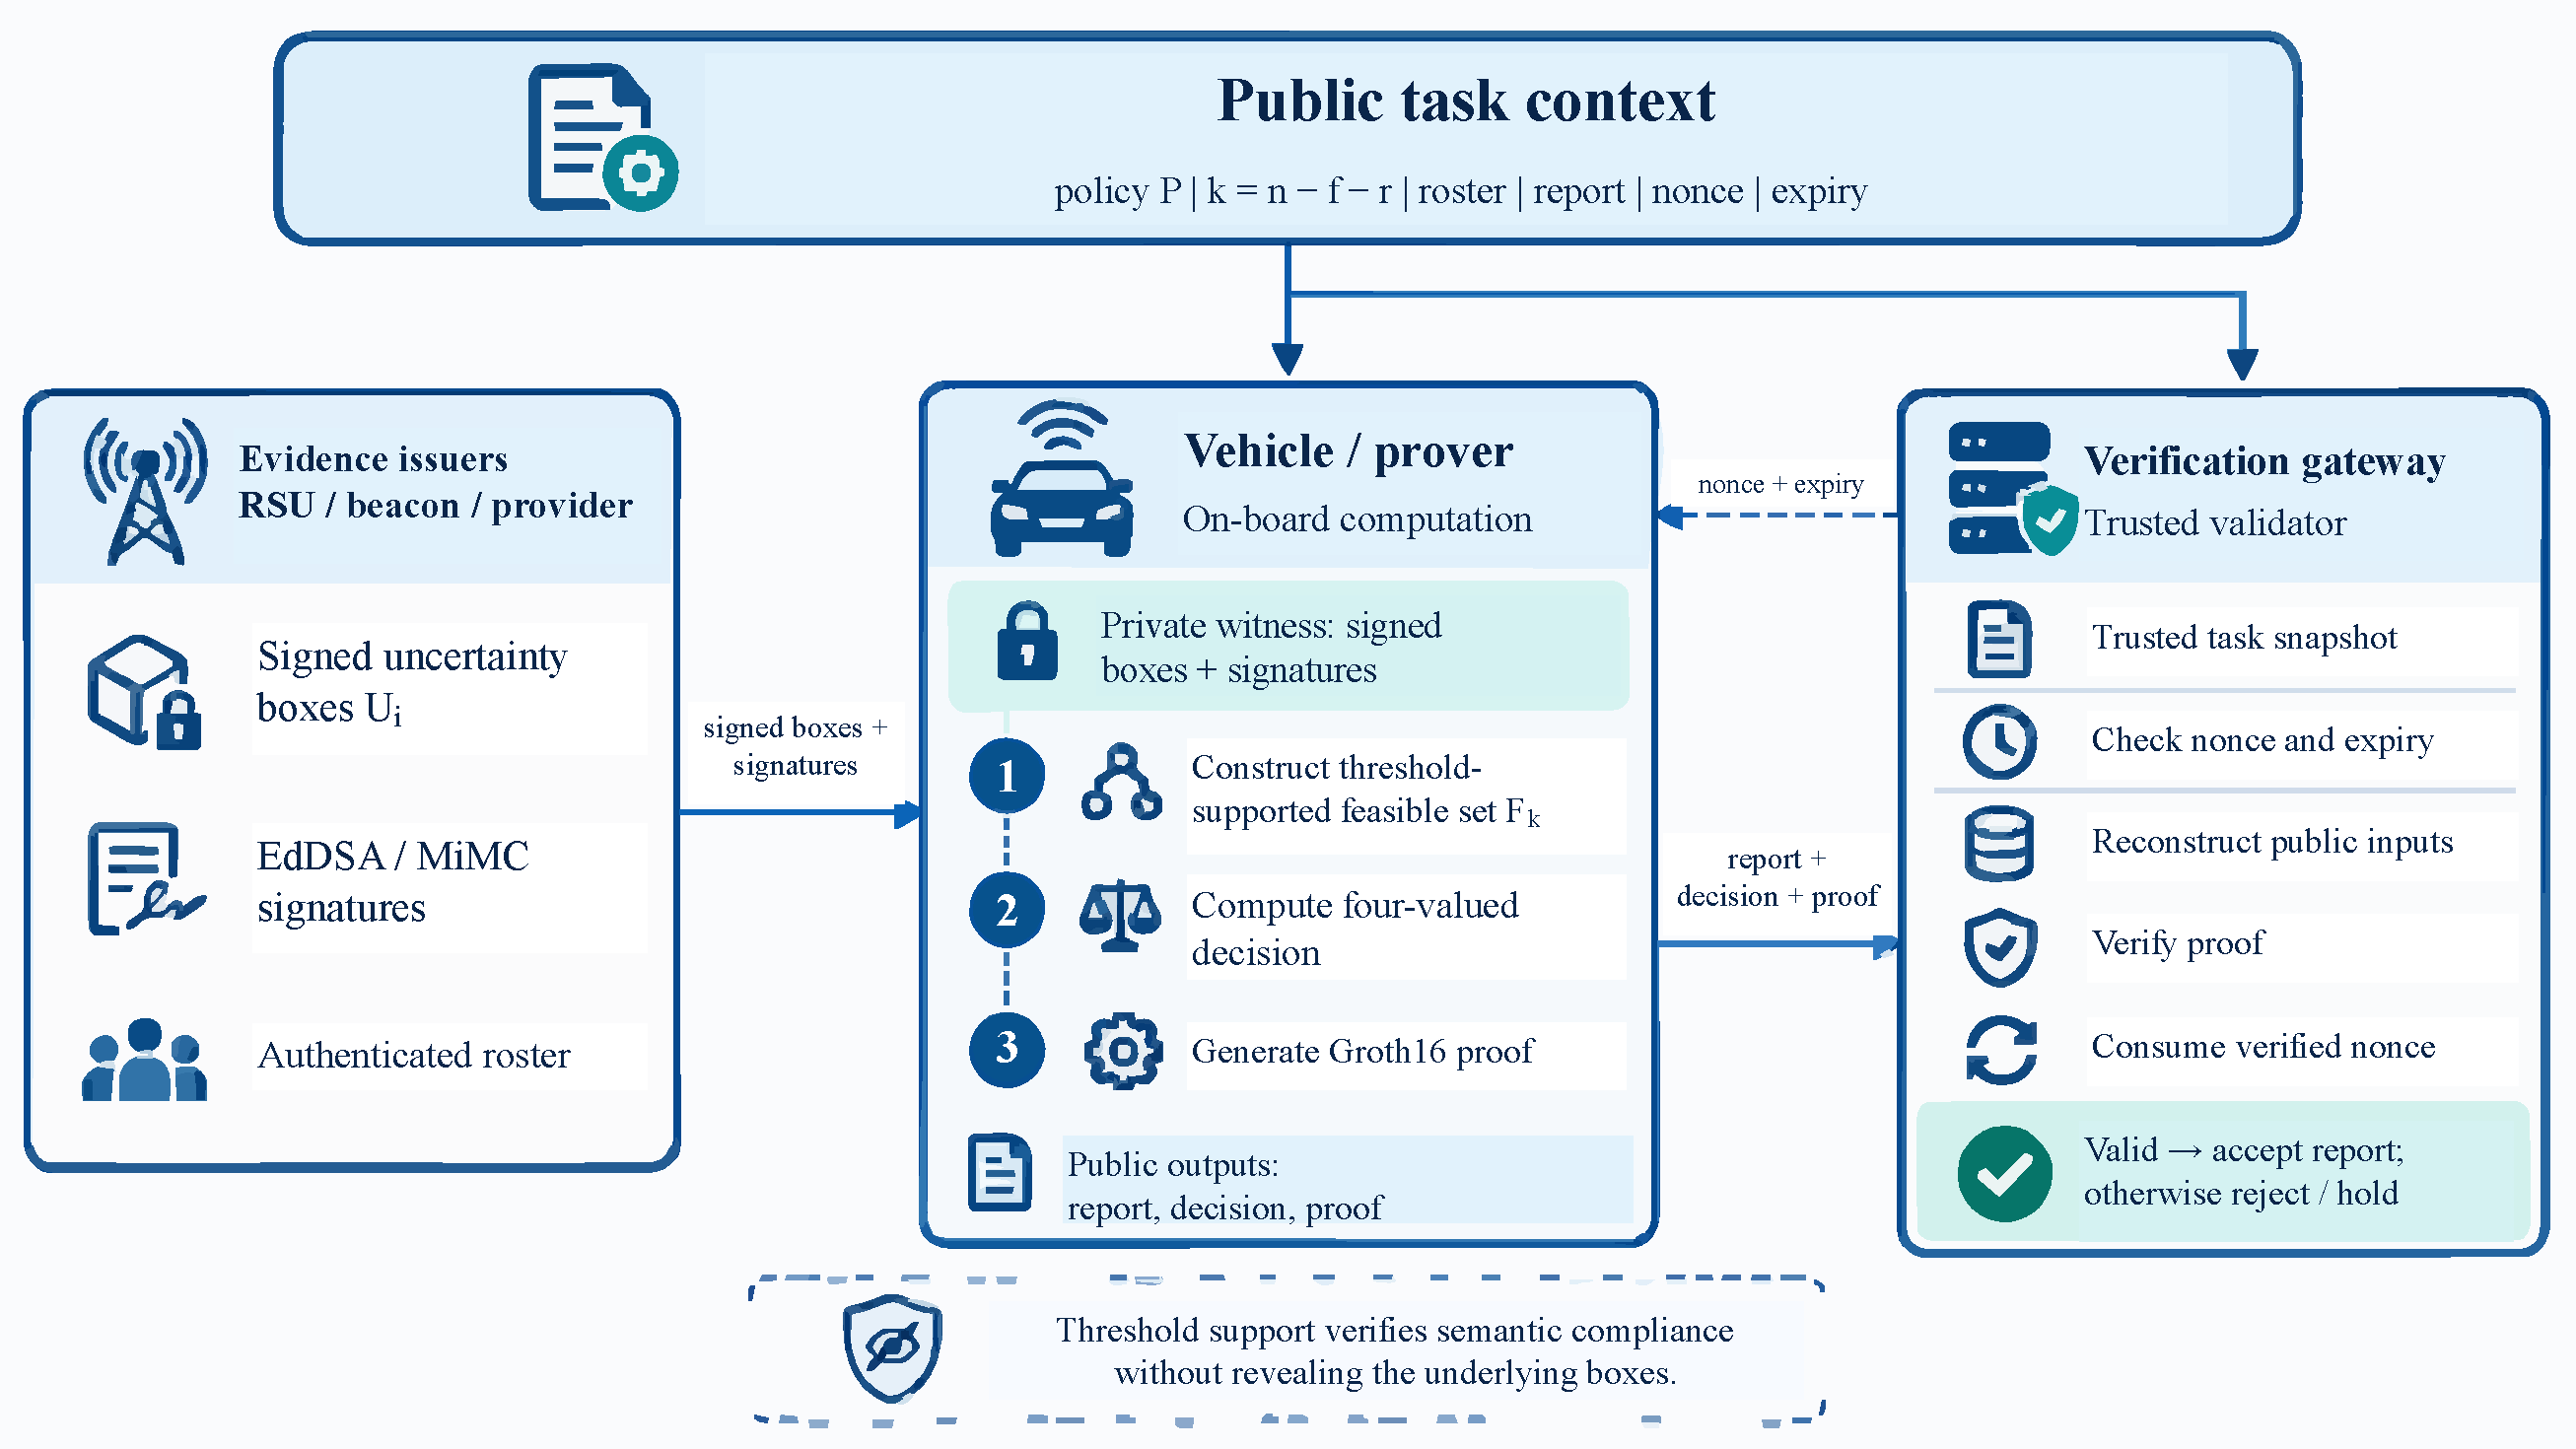
\includegraphics[width=\linewidth]{system_architecture.pdf}
\caption{Conceptual architecture of the evidence-certification module. Signed boxes $U_i$ contribute to the threshold-supported feasible set $\mathcal{F}_k$ in a quantized integer domain. An inconsistent decision represents a semantic outcome over complete, authenticated evidence, whereas missing or malformed evidence aborts the protocol. This schematic was generated with AI assistance (OpenAI ChatGPT).}\label{fig:architecture}
\end{figure}

Section 2 reviews relevant work on vehicular privacy, zero-knowledge location verification, and Byzantine-robust fusion. Section 3 develops the model and circuits; Section 4 establishes their security boundary; Section 5 presents the experiments; Section 6 discusses deployment and interoperability, and Section 7 concludes.